\documentclass[11pt]{article}
\usepackage[utf8]{inputenc}
\usepackage{graphicx}
\usepackage{verbatim}
\usepackage{listings}
\usepackage{mathtools}
\lstset{language=C, frame=single}

\topmargin=-15mm
\oddsidemargin=0mm
\textwidth=159.2mm
\textheight=220mm

\title{Home Exam 3: Video Encoding on GPU using the CUDA framework}
\author{Paweł Kozłowski \and Łukasz Mazurek}

\begin{document}
\maketitle
\pagebreak
\tableofcontents
\pagebreak

\section{Introduction}
In order to achieve the best efficiency of video encoding we made some optimizations of the following parts of the code:
\begin{itemize}
  \item Motion estimation,
  \item Motion compensation,
  \item DCT and quantize,
  \item VLC,
  \item Memory transfers.
\end{itemize}
Most of optimizations base on doing calculations on many \emph{CUDA} cores
in parallel.

\section{Motion estimation}

\subsection{Algorithm}
The first and the biggest bottleneck of the encoder is motion estimation.

\begin{figure}[h]
\centering
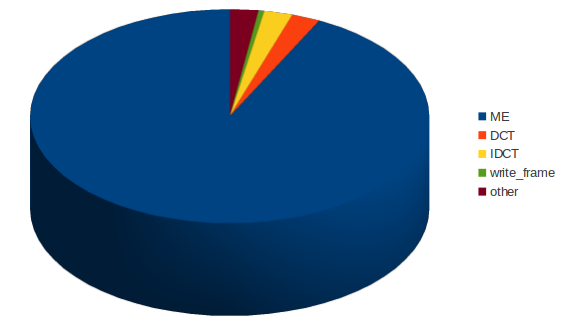
\includegraphics[width=0.5\textwidth]{images/precode.png}
\caption{Times of precode's parts}
\end{figure}

\noindent
There are plenty of algorithms faster than \emph{full search} to find the
motion vector using single-threaded architecture.
However, not all of them are well designed to use the potential of \emph{CUDA}.
Therefore we decided to optimize the \emph{full search} algorithm, since
it is very ``regular'' --- calculations for each non-border block looks exactly
the same (unlike in \emph{diamond search}).

\subsection{Division of tasks}
We can classify all the tasks among the 3 levels:
\begin{enumerate}
  \item The motion vector search is conducted for each $8 \times 8$ block 
  independently.
  For \texttt{tractor.yuv} movie, there are 32\,400 blocks to process.
  \item For each block, the task is to calculate $32 \cdot 32$ \emph{SAD} 
  functions and find the minimum of them.
  \item The calculating of a \emph{SAD} functions base on calculating 
  64 absolute differences between pixels values and summing up all the result.
\end{enumerate}

Ad. 3. Since the calculating of \emph{SAD} is a sequential task, we decided, that each \emph{SAD} is calculated by one thread.

Ad. 2. Each of $32 \cdot 32$ \emph{SAD} functions are calculated between the
particular block of original frame, and different blocks of reference frame.
Therefore it's a good task for one block of threads.
Unfortunately, we cannot use $32 \cdot 32$ threads on one block.
On \emph{Clinton} we are limited to 512 threads per thread block, 1024 threads and 8 thread blocks per one multiprocessor.
Therefore, to achieve the maximum occupancy of \emph{GPU} cores, we use 128
threads per a block, which leads to 1024 threads per a multiprocessor.
Thus, each of 128 threads must calculate 8 \emph{SAD} functions and find 
minimal value of them.
After that we can find the minimal \emph{SAD} among these 128 values using
\texttt{atomicMin()} function on a \emph{shared memory}.

Ad. 1. Each $8 \times 8$ block of frame is processed by a separate thread
block.

\subsection{Using of shared memory}
Each block of threads is calculating \emph{SAD} functions between one 
$8 \times 8$ block of original frame and $32 \times 32$ blocks of reference
frame. In order to do this, it needs $8 \times 8$ pixels from original
frame and $39 \times 39$ pixels from reference frame.
The kernel can read this data once from a global memory, store in shared
memory (which is much faster) and then use only shared memory for calculations.

\subsubsection{Transferring data from global to shared memory}
Since the transfer of data from global to shared memory takes noticeable amount
of time, it is important to do it efficiently in parallel using \emph{CUDA}
threads. 

Since we have 128 threads (16 rows of 8 threads each), we can read the
original frame block of 64 pixels in one command (using 64 threads).
However to provide parallel processing of this command we must avoid the bank
conflicts on a shared memory. In order to to this we figured out the pattern
of assigning the pixels to threads which avoids the bank conflicts in both
meanings (1.3 and 2.1 compute capabilities).

Besides the original frame block, each thread block needs to read 
$39 \cdot 39 = 1521$ pixels of reference data. We divided this area into
4 subareas shown in the picture.

The A area is being read in 8 commands by each of 128 threads.
The B (RIGHT) area is being read in 4 commands by each of 64 threads.
The C (BOTTOM) area is being read in 2 commands by each of 128 threads.
The D area is being read in 1 command by each of 64 threads.

In order to avoid the bank conflicts, we set the width of the array to 48,
and assigned the threads to the pixels as shown in the picture

\subsubsection{Calculating the SAD}
Since we have 128 threads and 1024 \emph{SAD} functions to calculate, each
thread must calculate 8 \emph{SAD}s. In this part we also figured out the
mapping between pixels and threads, which avoids the bank conflicts.

\begin{figure}[h]
\centering
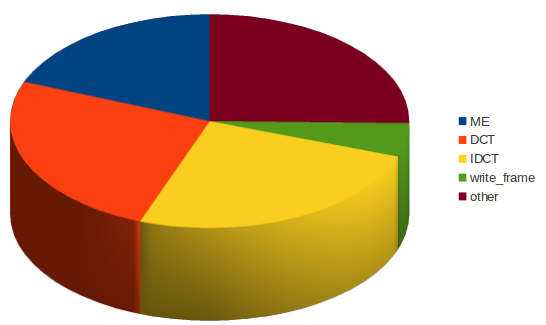
\includegraphics[width=0.5\textwidth]{images/cuda_me.png}
\caption{Times of precode's parts with ME on CUDA}
\end{figure}

\section{DCT/IDCT and quantization/dequantization}
Port of code which was computing \emph{DCT} and quantization was straight forward in the beginning. Of course first try of porting code to \emph{CUDA} resulted in slower runtime, because of a big number of useless uncoalesced global memory accessing. There is individual kernel per DCT/IDCT per Y/U/V frame, so in general there are run 6 kernels per one frame of video. We started to optimize it architecture-specific as below.

\subsection{Algorithm}
We used algorithm from precode with few modifications which were good for \emph{CUDA}.

\subsection{Division of tasks}
To lower the uncoalesced accessing each pair of macroblocks in a row is now computed by thread block (with 128 threads). So one half-warp with 16 threads reads 16 bytes in a row from global memory and copy it straight to shared memory without bank conflicts (there are 16 banks). Unfortunately because of another order of output data this is not true for writing to global memory. There is similar situation with \emph{IDCT}, just the opposite.

\subsection{Using of shared memory}
For computation specific for one macroblock we are using shared memory. We tried to avoid as many bank conflicts as possible to get higher performance. There are few places where are still bank conflicts but no better idea came to our minds. We were able to discard transposition of matrices thanks to putting result of multiplying \texttt{input} row by \texttt{dctlookup} column to appropriate place where it would be after transposition. Thanks to that we could lower even more the number of bank conflicts too. Really hard (or even impossible) part to avoid bank conflicts is quantization, we left it as it was. All of constant tables we put in constant memory on device.

\begin{figure}[h]
\centering
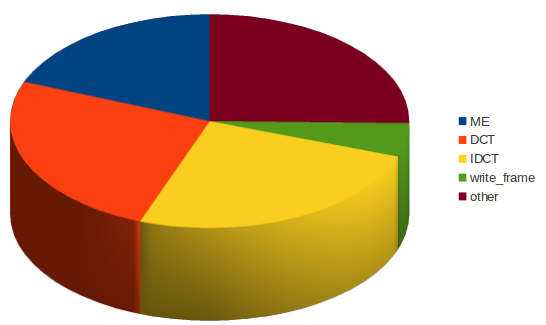
\includegraphics[width=0.5\textwidth]{images/cuda_me.png}
\caption{Times with ME and DCT/IDCT on CUDA}
\end{figure}

\section{VLC}
In the beginning \emph{VLC} was consuming a very little amount of time but after all other optimizations it was taking about 10\% of runtime. In the beginning we were trying to port whole \emph{VLC} to \emph{CUDA}, but after that we had understood its code very well, we did not have any idea to make it parallel because of its sequential nature. We decided in the end use CPU thread for writing output, because it can be done during computing \emph{CUDA} kernel on the device. Thanks to this optimization \emph{VLC} code is now running 3 times faster.

\section{Memory transfers}
Since we were porting the code of \emph{ME} and \emph{DCT} partially from 
\emph{CPU} to \emph{GPU}, after optimizations of these parts, the transfers
of data between \emph{host} and \emph{device} became signifact.

Each frame of data was being encoded in the following way:
\begin{itemize}
  \item reading of image by \emph{CPU},
  \item transfer of original and reference frame from \emph{host} to 
  \emph{device},
  \item motion estimation on \emph{GPU},
  \item transfer of calculated motion vectors to \emph{host},
  \item motion compesation on \emph{CPU},
  \item transfer of original and predicted frame to \emph{device},
  \item DCT and quantization on \emph{GPU},
  \item transfer of calculated residuals to \emph{host},
  \item transfer of residuals and prediction to \emph{device},
  \item quantization on \emph{GPU},
  \item transfer of reference frame to \emph{host},
  \item VLC and writing image on \emph{CPU}.
\end{itemize}
\pagebreak

\begin{figure}[h]
\centering
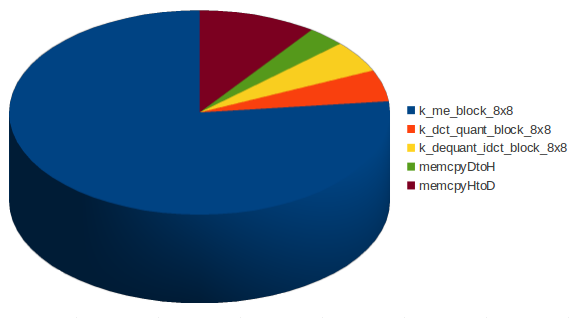
\includegraphics[width=0.5\textwidth]{images/before_all_device.png}
\caption{Times of kernels before reducing number of host $\leftrightarrow$ device memory transfers}
\end{figure}

After porting the motion compensation code to \emph{GPU}, the only things
which we have to do on \emph{CPU} were:
\begin{itemize}
  \item reading of image,
  \item VLC,
  \item writing the output.
\end{itemize}
Therefore we reduced the data transfers between the parts of encoding:
\begin{itemize}
  \item reading of frame on \emph{CPU},
  \item transfer of frame from \emph{host} to \emph{device},
  \item motion estimation and motion compensation on \emph{GPU},
  \item DCT, quantization, dequantization and IDCT on \emph{GPU},
  \item transfer of residuals and motion vectors to \emph{host},
  \item VLC and writing on \emph{CPU} being processed in parallel with
  encoding of the next frame.
\end{itemize}

\begin{figure}[h]
\centering
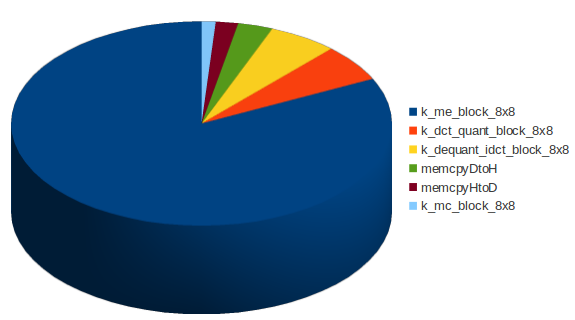
\includegraphics[width=0.5\textwidth]{images/after_all_device.png}
\caption{Times of kernels after reducing number of host $\leftrightarrow$ device memory transfers}
\end{figure}

\section{Summary}
To sum up video encoding task is very good to optimize with \emph{CUDA}. There is a lot of parts of code which can be run in parallel (in general all of them besides \emph{VLC}). Although, one needs to know architecture very well to write really good optimized code, it is not that hard thing because the architecture is very clear and well documented. Below we represent results of our work!

\begin{table}[h]
\centering
\begin{tabular}{|l|r|}
\hline
precode & 2200.69\,s \\
\hline
precode, ME on CUDA & 183.54\,s \\
\hline
ME and DCT/IDCT on CUDA & 74.66\,s \\\hline
reduced memory host $\leftrightarrow$ device transfers & 63.48\,s \\
\hline
thread for VLC & 53.41\,s \\
\hline
\end{tabular}
\caption{Times of encoding whole tractor.yuv with particular optimizations}
\end{table}

\end{document}
